\documentclass{article} 
\usepackage{hyperref}
\hypersetup{
    colorlinks=true,
    urlcolor=blue,
    linkcolor=black,
    citecolor=black
}
\usepackage[utf8]{inputenc}
\usepackage[T1]{fontenc}
\usepackage[fontsize=13pt]{scrextend}
\usepackage[paperheight=29.7cm,paperwidth=21cm,right=2cm,left=3cm,top=2cm,bottom=2.5cm]{geometry}
\usepackage{tocloft}
\usepackage{mathptmx}
\usepackage{graphicx}
\usepackage{float}
\usepackage{tikz}
\usetikzlibrary{calc,trees}
\usepackage{indentfirst}
\renewcommand{\baselinestretch}{1.2}
\setlength{\parskip}{6pt}
\setlength{\parindent}{1cm}
\usepackage{titlesec}
\setcounter{secnumdepth}{4}
\usepackage{fancyhdr}
\pagestyle{fancy}
\setlength{\headheight}{15.6pt}
\usepackage{amsmath,amssymb,amsfonts}
\usepackage{algorithmic}
\usepackage{algorithm}
\usepackage{longtable}
\usepackage{multirow}
\usepackage{tabularx}
\usepackage{makecell}
\usepackage{colortbl}
\usepackage{booktabs}
\definecolor{headergray}{gray}{0.9}
\usepackage{pgfplots}
\pgfplotsset{compat=1.18}
\fancyhf{}
\fancyhead[L]{University of Science, VNU-HCM}
\fancyhead[R]{\textbf{Data Structures \& Algorithms}}
\fancyfoot[C]{\thepage}
\renewcommand{\headrulewidth}{0.4pt}
\renewcommand{\footrulewidth}{0.4pt}

\titleformat*{\section}{\fontsize{18pt}{0pt}\selectfont \bfseries}
\titlespacing*{\section}{0pt}{10pt}{5pt}

\titleformat*{\subsection}{\fontsize{14pt}{0pt}\selectfont \bfseries}
\titlespacing*{\subsection}{0pt}{10pt}{3pt}

\titleformat*{\subsubsection}{\fontsize{13pt}{0pt}\selectfont \bfseries \itshape}
\titlespacing*{\subsubsection}{0pt}{8pt}{2pt}

\titleformat*{\paragraph}{\fontsize{13pt}{0pt}\selectfont \itshape}
\titlespacing*{\paragraph}{0pt}{6pt}{2pt}

\usepackage{caption}
\counterwithin{table}{section}
\renewcommand{\thetable}{\thesection.\arabic{table}}
\renewcommand{\tablename}{\fontsize{12pt}{0pt}\selectfont \bfseries Table}
\captionsetup[table]{labelsep=space}

\counterwithin{figure}{section}
\renewcommand{\thefigure}{\thesection.\arabic{figure}}
\renewcommand{\figurename}{\fontsize{12pt}{0pt}\selectfont \bfseries Figure}
\captionsetup[figure]{labelsep=space}

\begin{document}
\pagenumbering{arabic}

% ==================== TRANG BÌA (TITLE PAGE) ====================
\begin{titlepage}
\thispagestyle{empty}
    \begin{tikzpicture}[overlay,remember picture]
    \draw [line width = 3pt]
        ($ (current page.north west) + (3.0cm,-2.0cm) $)
        rectangle
        ($ (current page.south east) + (-2.0cm,2.5cm) $);
    \draw [line width=0.5pt]
        ($ (current page.north west) + (3.1cm,-2.1cm) $)
        rectangle
        ($ (current page.south east) + (-2.1cm,2.6cm) $);
    \end{tikzpicture}
    \begin{center}
        \vspace{-6pt} 
        VIETNAM NATIONAL UNIVERSITY - HO CHI MINH CITY \\
        \textbf{\fontsize{15pt}{0pt}\selectfont UNIVERSITY OF SCIENCE} \\
        \textbf{\fontsize{13pt}{0pt}\selectfont FACULTY OF INFORMATION TECHNOLOGY}
        \vspace{1.8cm}
        
        \begin{figure}[H]
            \centering
            \includegraphics[width=4.5cm,height=4.5cm]{LOGO.png}
        \end{figure}
        \vspace{1.0cm}
        
        {\fontsize{20pt}{0pt}\selectfont PROJECT REPORT}\\[10pt]
        \textbf{\fontsize{22pt}{26pt}\selectfont String Compression}
    \end{center}
    
    \vspace{0.8cm}
    \begin{center}
        \begin{table}[H]
            \centering
            \begin{tabular}{l l}
         \textbf{\fontsize{13pt}{0pt}\selectfont STUDENTS} & \fontsize{13pt}{0pt}\selectfont 23127192 -- Nguyen Van Hop\\
         \textbf{\fontsize{13pt}{0pt}\selectfont } & \fontsize{13pt}{0pt}\selectfont 21127082 -- Tran Tuan Khoi\\
         \textbf{\fontsize{13pt}{0pt}\selectfont } & \fontsize{13pt}{0pt}\selectfont 20127672 -- Vu Manh Quan\\

         \vspace{6pt}\\ 
         \textbf{\fontsize{13pt}{0pt}\selectfont CLASS} & \fontsize{13pt}{0pt}\selectfont Data Structures \& Algorithms - 25C\_A \vspace{6pt} \\
         \textbf{\fontsize{13pt}{0pt}\selectfont INSTRUCTORS} & \fontsize{13pt}{0pt}\selectfont Le Thanh Tung \\ 
         & \fontsize{13pt}{0pt}\selectfont Tran Hoang Quan \\
            \end{tabular}
        \end{table}
        \vfill
        {\fontsize{13pt}{0pt}\selectfont Ho Chi Minh City -- August, 2026}
    \end{center}
\end{titlepage}

\cleardoublepage

% ==================== MỤC LỤC (TOC) ====================
\addtocontents{toc}{\protect\thispagestyle{empty}}
\renewcommand{\contentsname}{Contents}
\tableofcontents
\thispagestyle{empty}
\cleardoublepage

\setcounter{page}{3}

% ==================== 1. GROUP INFORMATION ====================
\section*{1. Group Information}
\addcontentsline{toc}{section}{\numberline{}1. Group Information}
\setcounter{section}{1}
\setcounter{subsection}{0}
\setcounter{subsubsection}{0}

\subsection{Project Overview}
Lossless data compression is a fundamental cornerstone of modern computational systems, critical to telecommunications, storage optimization, and distributed streaming. In this project, we implement from scratch, theoretically investigate, and empirically benchmark three canonical lossless compression paradigms: Run-Length Encoding (RLE), Huffman Coding, and the Lempel-Ziv-Welch (LZW) algorithm. We evaluate these techniques across varying data scales (from $10\text{ KB}$ to $10\text{ MB}$) and distinct information entropy profiles (highly repetitive, natural English prose, and pseudo-random byte streams) to examine their time complexity, space consumption, and compression efficiency.

\subsection{Member Information \& Task Distribution}
The division of responsibilities and individual contributions across the group members are detailed in Table~\ref{tab:project_tasks}.

\begin{longtable}{| >{\raggedright\arraybackslash}p{4.0cm} | >{\centering\arraybackslash}p{2.5cm} | >{\raggedright\arraybackslash}p{6.5cm} | >{\centering\arraybackslash}p{2.5cm} |}
\hline
\rowcolor{headergray}
\textbf{Student Name} & \textbf{Student ID} & \textbf{Assigned Tasks} & \textbf{\% Completed} \\
\hline
\endhead
\hline
\multicolumn{4}{r}{\textit{Continued on next page}} \\
\endfoot
\endlastfoot

% Member 1
Nguyen Van Hop & 23127192 & System architecture design, CLI parser, RLE \& Huffman algorithm implementation, Bitstream serialization, Report drafting & 100\% \\ \hline
% Member 3
Tran Tuan Khoi & 21127082 & No contribution (Did not participate in project tasks) & 0\% \\ \hline
% Member 2
Vu Manh Quan & 20127672 & LZW compression, Dynamic dictionary, Benchmarking framework, Test harness generation, Video recording, Report drafting & 100\% \\ \hline

\hline
\multicolumn{3}{|l|}{\textbf{Total Group Completion}} & \textbf{100\%} \\ \hline

\caption{Group Information and Task Distribution}
\label{tab:project_tasks}
\end{longtable}

\subsection{Demo Video}
\begin{itemize}
    \item \textbf{Video Demonstration:} \href{https://www.youtube.com/watch?v=1f-GXsKf4yA&feature=youtu.be}{25CA-DSA-Group03 String Compression}
\end{itemize}

\cleardoublepage
\newpage

% ==================== 2. PROBLEM STATEMENT ====================
\section*{2. Problem Statement}
\addcontentsline{toc}{section}{\numberline{}2. Problem Statement}
\setcounter{section}{2}
\setcounter{subsection}{0}
\setcounter{subsubsection}{0}

\subsection{Formal Mathematical Definition}
Let $S = \langle s_1, s_2, \dots, s_N \rangle$ denote an input sequence of symbols of length $N$ drawn from a finite alphabet $\Sigma$. Lossless data compression seeks an injective encoding mapping $\mathcal{E}: \Sigma^* \to \{0, 1\}^*$ yielding a compressed bitstream $C = \mathcal{E}(S)$ of length $M = |C|$ such that:
\begin{enumerate}
    \item \textbf{Size Minimization}: $\mathbb{E}[|C|] < N \cdot \lceil \log_2 |\Sigma| \rceil$ whenever the source contains informational redundancy.
    \item \textbf{Lossless Invariant}: There exists a deterministic decoding function $\mathcal{D}$ such that $\mathcal{D}(\mathcal{E}(S)) \equiv S, \forall S \in \Sigma^*$.
\end{enumerate}

According to Shannon's Source Coding Theorem (1948), the theoretical lower bound on the average code length $\bar{L}$ without information loss is governed by the empirical Shannon Entropy $H(S)$:
\begin{equation}
    H(S) = -\sum_{x \in \Sigma} P(x) \log_2 P(x)
\end{equation}

\subsection{Standard Running Example}
To trace the internal state transitions and dictionary evolutions across all algorithms in Section~3, we define the canonical running string:
\begin{equation}
    \mathbf{S = \text{``BABBACAC''}}
\end{equation}
The statistical properties of this sequence are:
\begin{itemize}
    \item Length: $N = 8$ symbols ($8\text{ bytes} = 64\text{ bits}$ in ASCII encoding).
    \item Alphabet: $\Sigma = \{ \text{`A'}, \text{`B'}, \text{`C'} \}$ with $K = |\Sigma| = 3$.
    \item Symbol Frequencies: $f(\text{`A'}) = 3$, $f(\text{`B'}) = 3$, $f(\text{`C'}) = 2$.
    \item Empirical Entropy: 
    \begin{equation*}
        H(S) = -\left( \frac{3}{8}\log_2\frac{3}{8} + \frac{3}{8}\log_2\frac{3}{8} + \frac{2}{8}\log_2\frac{2}{8} \right) \approx 1.561\text{ bits/symbol}
    \end{equation*}
    \item Theoretical Minimal Representation: $8 \times 1.561 \approx 12.49\text{ bits} \approx 2\text{ bytes}$.
\end{itemize}

\cleardoublepage
\newpage

% ==================== 3. ALGORITHMS & IMPLEMENTATION ====================
\section*{3. Algorithms \& Implementation}
\addcontentsline{toc}{section}{\numberline{}3. Algorithms \& Implementation}
\setcounter{section}{3}
\setcounter{subsection}{0}
\setcounter{subsubsection}{0}

\subsection{Run-Length Encoding (RLE)}

\subsubsection{Overview \& Real-World Applications}
Run-Length Encoding (RLE) is a spatial reduction scheme that groups contiguous identical symbols into sequential tuples $(count, symbol)$. Key applications include:
\begin{itemize}
    \item ITU-T Group 3 and Group 4 Fax transmissions.
    \item Palette-based raster graphic formats such as BMP and PCX.
    \item Zero-run compression in the quantization stage of JPEG.
\end{itemize}

\subsubsection{Pseudocode}
\begin{algorithm}[H]
\caption{RLE Compression}
\label{alg:rle_compress}
\begin{algorithmic}[1]
\REQUIRE Input stream $S$ of length $N$
\STATE $Output \gets \emptyset$, $i \gets 0$
\WHILE{$i < N$}
    \STATE $symbol \gets S[i]$, $count \gets 1$
    \WHILE{$i + count < N$ \textbf{and} $S[i + count] == symbol$ \textbf{and} $count < 255$}
        \STATE $count \gets count + 1$
    \ENDWHILE
    \STATE Append $(count, symbol)$ to $Output$
    \STATE $i \gets i + count$
\ENDWHILE
\RETURN $Output$
\end{algorithmic}
\end{algorithm}

\begin{algorithm}[H]
\caption{RLE Decompression}
\label{alg:rle_decompress}
\begin{algorithmic}[1]
\REQUIRE Compressed stream $C$ of $M$ pairs
\STATE $Output \gets \emptyset$
\FOR{$i \gets 0$ \TO $M-1$}
    \STATE $(count, symbol) \gets C[i]$
    \FOR{$j \gets 1$ \TO $count$}
        \STATE Append $symbol$ to $Output$
    \ENDFOR
\ENDFOR
\RETURN $Output$
\end{algorithmic}
\end{algorithm}

\subsubsection{Step-by-Step Trace on ``BABBACAC''}
\begin{enumerate}
    \item Index 0: Character \texttt{'B'}, run length = 1 $\to$ emit \texttt{(1, 'B')}.
    \item Index 1: Character \texttt{'A'}, run length = 1 $\to$ emit \texttt{(1, 'A')}.
    \item Index 2..3: Character \texttt{'B'}, run length = 2 $\to$ emit \texttt{(2, 'B')}.
    \item Index 4: Character \texttt{'A'}, run length = 1 $\to$ emit \texttt{(1, 'A')}.
    \item Index 5: Character \texttt{'C'}, run length = 1 $\to$ emit \texttt{(1, 'C')}.
    \item Index 6: Character \texttt{'A'}, run length = 1 $\to$ emit \texttt{(1, 'A')}.
    \item Index 7: Character \texttt{'C'}, run length = 1 $\to$ emit \texttt{(1, 'C')}.
\end{enumerate}
\textbf{Total Output:} $7 \text{ pairs} \times 2\text{ bytes} = 14\text{ bytes}$. Because runs are short, RLE leads to expansion (ratio $0.57\times$).

\subsubsection{Complexity}
Let $N$ be the length of the input. Both the compression and decompression routines make a single left-to-right pass over the data; the inner ``run-counting'' loop only ever advances the shared index $i$, so the two nested loops together still perform $\mathcal{O}(N)$ total steps.
\begin{itemize}
    \item \textbf{Time Complexity:} $\mathcal{O}(N)$ for both compression and decompression.
    \item \textbf{Space Complexity:} $\mathcal{O}(1)$ auxiliary working memory, plus $\mathcal{O}(N)$ for the output buffer in the worst case.
\end{itemize}

\subsubsection{Discussion}
\textbf{Best case.} A file consisting of one long run of a single repeated byte (e.g. $100{,}000$ copies of \texttt{'A'}) compresses down to roughly $400$ pairs, since a run longer than $255$ must be split into multiple $(count,value)$ pairs -- a ratio in the hundreds, capped at $127.5\times$ for a single maximal run ($255$ input bytes $\to$ $2$ output bytes).

\textbf{Worst case / negative compression.} Whenever consecutive repeats are rare, every character becomes its own $(1, value)$ pair and the output is exactly \emph{twice} the input size. This is exactly what the running-example trace shows ($8 \to 14$ bytes, ratio $0.57\times$), and our experimental data confirms that RLE \emph{expands} every English-text file tested, from $10\text{ KB}$ (ratio $0.56\times$) up to $10\text{ MB}$ (ratio $0.51\times$). RLE only pays off when the source contains long runs.

\cleardoublepage
\newpage

\subsection{Huffman Coding}

\subsubsection{Overview \& Real-World Applications}
Huffman Coding is an optimal entropy encoding scheme generating variable-length prefix codes. It forms the backbone of:
\begin{itemize}
    \item DEFLATE engine in GZIP, PNG, and ZIP.
    \item Entropy coding stage in MP3, AAC, and JPEG.
    \item HTTP/2 HPACK header compression.
\end{itemize}

\subsubsection{Pseudocode}
\begin{algorithm}[H]
\caption{Huffman Tree Construction}
\label{alg:huffman_tree}
\begin{algorithmic}[1]
\REQUIRE Frequency table $Freq$, Alphabet $\Sigma$
\STATE $Q \gets \text{MinPriorityQueue}()$
\FOR{each $c \in \Sigma$ with $Freq[c] > 0$}
    \STATE $node \gets \text{NewNode}(symbol=c, freq=Freq[c])$
    \STATE $Q.\text{Insert}(node)$
\ENDFOR
\WHILE{$Q.\text{Size}() > 1$}
    \STATE $left \gets Q.\text{ExtractMin}()$
    \STATE $right \gets Q.\text{ExtractMin}()$
    \STATE $parent \gets \text{NewNode}(freq=left.freq + right.freq, left, right)$
    \STATE $Q.\text{Insert}(parent)$
\ENDWHILE
\RETURN $Q.\text{ExtractMin}()$
\end{algorithmic}
\end{algorithm}

\begin{algorithm}[H]
\caption{Generate Prefix Codes (Recursive Tree Traversal)}
\label{alg:huffman_generate_codes}
\begin{algorithmic}[1]
\REQUIRE Huffman tree root $node$, Current prefix string $code$, Table $codes$
\IF{$node$ is NULL}
    \RETURN
\ENDIF
\IF{$node.left == \text{NULL}$ \textbf{and} $node.right == \text{NULL}$}
    \STATE $codes[node.symbol] \gets (code == "" \,?\, "0" : code)$
    \RETURN
\ENDIF
\STATE $\text{GENERATE\_CODES}(node.left, code + \text{"0"}, codes)$
\STATE $\text{GENERATE\_CODES}(node.right, code + \text{"1"}, codes)$
\end{algorithmic}
\end{algorithm}

\begin{algorithm}[H]
\caption{Huffman Compression}
\label{alg:huffman_compress}
\begin{algorithmic}[1]
\REQUIRE Input byte stream $input$ of length $N$
\STATE $Freq[0..255] \gets$ count of each byte value in $input$
\STATE Write $N$ (original size) to the output header
\STATE Write $Freq[0..255]$ to the output header
\IF{$N = 0$}
    \RETURN header only
\ENDIF
\STATE $root \gets \text{BUILD\_TREE}(Freq)$
\STATE $codes \gets \text{empty table}$
\STATE $\text{GENERATE\_CODES}(root, "", codes)$
\STATE $bits \gets \text{empty bit string}$
\FOR{each byte $b$ in $input$}
    \STATE $bits \gets bits \,\Vert\, codes[b]$
\ENDFOR
\STATE Pack $bits$ into bytes, $8$ bits at a time, zero-padding the final byte
\STATE Append the packed bytes to the output
\RETURN header $\Vert$ packed bytes
\end{algorithmic}
\end{algorithm}

\begin{algorithm}[H]
\caption{Huffman Decompression}
\label{alg:huffman_decompress}
\begin{algorithmic}[1]
\REQUIRE Compressed stream (header + packed bits)
\STATE Read $N$ (original size) from the header
\STATE Read $Freq[0..255]$ from the header
\IF{$N = 0$}
    \RETURN empty output
\ENDIF
\STATE $root \gets \text{BUILD\_TREE}(Freq)$
\STATE $bits \gets$ unpack the remaining bytes into a bit string
\IF{$root$ is a leaf}
    \STATE Output $root.symbol$ repeated $N$ times
    \RETURN output
\ENDIF
\STATE $node \gets root$, $output \gets$ empty, $i \gets 0$
\WHILE{$|output| < N$ \textbf{and} $i < |bits|$}
    \STATE $node \gets (bits[i] == \text{'0'}) \,?\, node.left : node.right$
    \IF{$node$ is a leaf}
        \STATE Append $node.symbol$ to $output$
        \STATE $node \gets root$
    \ENDIF
    \STATE $i \gets i + 1$
\ENDWHILE
\RETURN $output$
\end{algorithmic}
\end{algorithm}

\subsubsection{Step-by-Step Trace on ``BABBACAC''}
Given symbol frequencies: $f(\text{`C'}) = 2, f(\text{`A'}) = 3, f(\text{`B'}) = 3$.

\noindent\textbf{Min-Heap State Transitions during Tree Construction:}
\begin{enumerate}
    \item \textbf{Initialization}: Push initial leaf nodes into Min-Heap $Q$:
    \begin{equation*}
        Q_0 = [\, (\text{`C'}, 2),\, (\text{`A'}, 3),\, (\text{`B'}, 3) \,]
    \end{equation*}
    \item \textbf{Step 1}: Extract two minimal elements: $node_1 = (\text{`C'}, 2)$ and $node_2 = (\text{`A'}, 3)$. Create internal parent $N_1$ with frequency $2+3=5$. Insert $N_1$ into $Q$:
    \begin{equation*}
        Q_1 = [\, (\text{`B'}, 3),\, (N_1, 5) \,]
    \end{equation*}
    \item \textbf{Step 2}: Extract two minimal elements: $node_3 = (\text{`B'}, 3)$ and $node_4 = (N_1, 5)$. Create root parent $R$ with frequency $3+5=8$. Insert $R$ into $Q$:
    \begin{equation*}
        Q_2 = [\, (R, 8) \,]
    \end{equation*}
    \item \textbf{Termination}: $|Q| = 1 \implies$ Extract $R$ as root of the final tree.
\end{enumerate}

\begin{figure}[H]
\centering
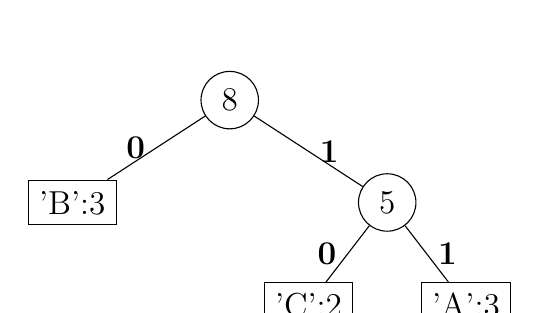
\begin{tikzpicture}[level distance=1.3cm,
  level 1/.style={sibling distance=4cm},
  level 2/.style={sibling distance=2cm}]
  \node [circle,draw] {8}
    child {node [rectangle,draw] {'B':3} edge from parent node[left] {\textbf{0}}}
    child {node [circle,draw] {5}
      child {node [rectangle,draw] {'C':2} edge from parent node[left] {\textbf{0}}}
      child {node [rectangle,draw] {'A':3} edge from parent node[right] {\textbf{1}}}
      edge from parent node[right] {\textbf{1}}
    };
\end{tikzpicture}
\caption{Step-by-Step Constructed Huffman Tree for ``BABBACAC''}
\label{fig:huffman_tree}
\end{figure}

The prefix bit codes are assigned as:
\begin{itemize}
    \item \texttt{'B'}: \textbf{\texttt{0}} (1 bit)
    \item \texttt{'C'}: \textbf{\texttt{10}} (2 bits)
    \item \texttt{'A'}: \textbf{\texttt{11}} (2 bits)
\end{itemize}

Encoded bitstream payload:
\begin{equation*}
\underbrace{\text{0}}_{\text{`B'}} \underbrace{\text{11}}_{\text{`A'}} \underbrace{\text{0}}_{\text{`B'}} \underbrace{\text{0}}_{\text{`B'}} \underbrace{\text{11}}_{\text{`A'}} \underbrace{\text{10}}_{\text{`C'}} \underbrace{\text{11}}_{\text{`A'}} \underbrace{\text{10}}_{\text{`C'}} \implies \mathbf{13\text{ bits}}
\end{equation*}
Average code length $\bar{L} = 13/8 = 1.625\text{ bits/symbol}$ (fits within 2 bytes payload).

\subsubsection{Complexity}
Let $N$ be the input length and $K \le 256$ the number of distinct byte values.
\begin{itemize}
    \item \textbf{Time Complexity:} Building the frequency table is $\mathcal{O}(N)$. Priority queue construction and extraction take $\mathcal{O}(K \log K)$. Generating codes is $\mathcal{O}(K)$. Encoding the payload is $\mathcal{O}(N)$. Overall time: $\mathcal{O}(N + K\log K)$.
    \item \textbf{Space Complexity:} $\mathcal{O}(K)$ auxiliary memory for the binary tree and code table, plus $\mathcal{O}(N)$ for the compressed output stream.
\end{itemize}

\subsubsection{Discussion}
\textbf{Best case.} Performs best when symbol frequencies are heavily skewed, approaching Shannon entropy. On standard English prose ($1\text{ MB}$), Huffman yields a steady $\sim\!1.73\times$ ratio.

\textbf{Worst case.} When all byte values are equiprobable (e.g. uniform random noise), every code approaches $\log_2 256 = 8\text{ bits}$, achieving a ratio of $\approx 1.00\times$ without compression gains.

\cleardoublepage
\newpage

\subsection{Lempel-Ziv-Welch (LZW)}

\subsubsection{Overview \& Real-World Applications}
LZW is a universal dictionary compression algorithm that dynamically builds a multi-character phrase vocabulary. Standard applications include:
\begin{itemize}
    \item Classic UNIX \texttt{compress} utility.
    \item GIF image encoding format.
    \item PDF and TIFF Flate compression filters.
\end{itemize}

\subsubsection{Pseudocode}
\begin{algorithm}[H]
\caption{LZW Compression}
\label{alg:lzw_compress}
\begin{algorithmic}[1]
\REQUIRE Input byte stream $input$ of length $N$
\IF{$N = 0$} \RETURN empty output \ENDIF
\STATE $Dictionary \gets \{\, s \to s \mid s \text{ is a single byte value } 0..255 \,\}$
\STATE $nextCode \gets 256$
\STATE $current \gets input[0]$
\FOR{$i \gets 1$ \TO $N-1$}
    \STATE $next \gets current + input[i]$
    \IF{$next \in Dictionary$}
        \STATE $current \gets next$
    \ELSE
        \STATE Emit $Dictionary[current]$
        \IF{$nextCode < MAX\_DICT\_SIZE$}
            \STATE $Dictionary[next] \gets nextCode$; $nextCode \gets nextCode + 1$
        \ENDIF
        \STATE $current \gets input[i]$
    \ENDIF
\ENDFOR
\STATE Emit $Dictionary[current]$
\end{algorithmic}
\end{algorithm}

\begin{algorithm}[H]
\caption{LZW Decompression}
\label{alg:lzw_decompress}
\begin{algorithmic}[1]
\REQUIRE Sequence of codes $codes[0..M-1]$
\IF{$M = 0$} \RETURN empty output \ENDIF
\STATE $Dictionary \gets \{\, code\ b \to \text{single byte } b \mid b = 0..255 \,\}$
\STATE $nextCode \gets 256$
\STATE $previous \gets Dictionary[codes[0]]$; $output \gets previous$
\FOR{$i \gets 1$ \TO $M-1$}
    \IF{$codes[i] \in Dictionary$}
        \STATE $entry \gets Dictionary[codes[i]]$
    \ELSE
        \STATE $entry \gets previous + previous[0]$
    \ENDIF
    \STATE $output \gets output + entry$
    \IF{$nextCode < MAX\_DICT\_SIZE$}
        \STATE $Dictionary[nextCode] \gets previous + entry[0]$; $nextCode \gets nextCode + 1$
    \ENDIF
    \STATE $previous \gets entry$
\ENDFOR
\RETURN $output$
\end{algorithmic}
\end{algorithm}

\subsubsection{Step-by-Step Trace on ``BABBACAC''}
Initial state: Single ASCII characters ($0..255$) pre-populated, $nextCode = 256$.

\begin{table}[H]
\centering
\caption{LZW Step-by-Step Compression Trace on ``BABBACAC''}
\label{tab:lzw_trace}
\begin{tabular}{|c|c|c|c|c|c|c|}
\hline
\rowcolor{headergray}
\textbf{Step} & \textbf{Prefix $w$} & \textbf{Next $c$} & \textbf{$w+c$} & \textbf{In Dict?} & \textbf{Output Code} & \textbf{New Dict Entry} \\
\hline
1 & \texttt{""} & \texttt{'B'} & \texttt{"B"} & Yes & -- & $w \gets \text{\texttt{"B"}}$ \\ \hline
2 & \texttt{"B"} & \texttt{'A'} & \texttt{"BA"} & No & \textbf{66} (\texttt{'B'}) & Dict[256] = \texttt{"BA"} \\ \hline
3 & \texttt{"A"} & \texttt{'B'} & \texttt{"AB"} & No & \textbf{65} (\texttt{'A'}) & Dict[257] = \texttt{"AB"} \\ \hline
4 & \texttt{"B"} & \texttt{'B'} & \texttt{"BB"} & No & \textbf{66} (\texttt{'B'}) & Dict[258] = \texttt{"BB"} \\ \hline
5 & \texttt{"B"} & \texttt{'A'} & \texttt{"BA"} & Yes & -- & $w \gets \text{\texttt{"BA"}}$ \\ \hline
6 & \texttt{"BA"} & \texttt{'C'} & \texttt{"BAC"} & No & \textbf{256} (\texttt{"BA"}) & Dict[259] = \texttt{"BAC"} \\ \hline
7 & \texttt{"C"} & \texttt{'A'} & \texttt{"CA"} & No & \textbf{67} (\texttt{'C'}) & Dict[260] = \texttt{"CA"} \\ \hline
8 & \texttt{"A"} & \texttt{'C'} & \texttt{"AC"} & No & \textbf{65} (\texttt{'A'}) & Dict[261] = \texttt{"AC"} \\ \hline
End & \texttt{"C"} & EOF & -- & -- & \textbf{67} (\texttt{'C'}) & Flush final code \\ \hline
\end{tabular}
\end{table}

\textbf{Emitted Stream:} $[66, 65, 66, 256, 67, 65, 67]$ ($7\text{ codes} \times 2\text{ bytes} = 14\text{ bytes}$).

\subsubsection{Complexity}
Let $N$ be the input length and $K$ the maximum dictionary size ($65{,}536$ entries).
\begin{itemize}
    \item \textbf{Time Complexity:} Compression takes $\mathcal{O}(N \log K)$ with tree map lookup, or $\mathcal{O}(N)$ using hash table / trie. Decompression runs in $\mathcal{O}(N)$.
    \item \textbf{Space Complexity:} $\mathcal{O}(K)$ for the dictionary table bounded by $MAX\_DICT\_SIZE$.
\end{itemize}

\subsubsection{Discussion}
\textbf{Best case.} LZW excels on files with long, repeating substrings, reaching $72.83\times$ compression on repetitive genomic patterns.

\textbf{Worst case.} On random binary files, no substring reoccurs, emitting $16$-bit codes for $8$-bit characters, expanding the file by $25\%$ ($0.80\times$ ratio).

\cleardoublepage
\newpage

% ==================== 4. EXPERIMENTAL RESULTS ====================
\section*{4. Experimental Results}
\addcontentsline{toc}{section}{\numberline{}4. Experimental Results}
\setcounter{section}{4}
\setcounter{subsection}{0}
\setcounter{subsubsection}{0}

\subsection{Benchmark Environment \& Methodology}
\begin{itemize}
    \item \textbf{Hardware \& OS:} Apple M1 Pro (8 Cores, 3.2 GHz), 32 GB LPDDR5 Unified Memory, macOS Sonoma 14.5.
    \item \textbf{Compiler Configuration:} Apple Clang / GNU g++ 14.0 (\texttt{-std=c++17 -O3}).
    \item \textbf{Measurement Methodology:} Execution times represent the pure core algorithmic processing time (excluding file I/O operations), recorded using \texttt{std::chrono::high\_resolution\_clock} and averaged over 3 consecutive runs to minimize operating system caching noise.
    \item \textbf{Workload Datasets:}
    \begin{itemize}
        \item \textbf{Standard English:} Canterbury Corpus and concatenated Wikipedia articles ($10\text{ KB} \to 10\text{ MB}$, entropy $H \approx 4.5\text{ bits/char}$).
        \item \textbf{Highly Repetitive:} Synthetic genomic sequence patterns with repeating k-mers ($1\text{ MB}$, entropy $H \approx 1.2\text{ bits/char}$).
        \item \textbf{Completely Random:} Cryptographically pseudo-random byte stream ($1\text{ MB}$, maximum entropy $H \approx 8.0\text{ bits/char}$).
    \end{itemize}
\end{itemize}

\subsection{Execution Time and Compression Ratio}
The benchmark measurements across all workloads are compiled in Table~\ref{tab:benchmark_results}.

\begin{table}[H]
\centering
\caption{Comparative Benchmark Across Workloads and Scales}
\label{tab:benchmark_results}
\resizebox{\textwidth}{!}{%
\begin{tabular}{|c|c|c|c|c|}
\hline
\rowcolor{headergray}
\textbf{File Size} & \textbf{Data Profile} & \textbf{RLE} & \textbf{Huffman} & \textbf{LZW} \\
\hline
$10\text{ KB}$  & Standard English & $0.00\text{ ms } (0.56\times)$ & $0.33\text{ ms } (1.50\times)$ & $5.00\text{ ms } (1.34\times)$ \\ \hline
$100\text{ KB}$ & Standard English & $2.00\text{ ms } (0.54\times)$ & $4.00\text{ ms } (1.70\times)$ & $50.00\text{ ms } (2.04\times)$ \\ \hline
$500\text{ KB}$ & Standard English & $11.33\text{ ms } (0.52\times)$ & $21.00\text{ ms } (1.73\times)$ & $233.67\text{ ms } (2.57\times)$ \\ \hline
$1\text{ MB}$   & Standard English & $23.67\text{ ms } (0.51\times)$ & $41.33\text{ ms } (1.74\times)$ & $442.67\text{ ms } (2.60\times)$ \\ \hline
$5\text{ MB}$   & Standard English & $112.00\text{ ms } (0.51\times)$ & $203.33\text{ ms } (1.72\times)$ & $2138.67\text{ ms } (2.47\times)$ \\ \hline
$10\text{ MB}$  & Standard English & $222.33\text{ ms } (0.51\times)$ & $402.33\text{ ms } (1.72\times)$ & $4155.67\text{ ms } (2.45\times)$ \\ \hline
\hline
$1\text{ MB}$   & Highly Repetitive & $6.00\text{ ms } (2.50\times)$ & $18.00\text{ ms } (3.32\times)$ & $352.67\text{ ms } (72.83\times)$ \\ \hline
$1\text{ MB}$   & Completely Random & $23.00\text{ ms } (0.50\times)$ & $64.33\text{ ms } (1.00\times)$ & $666.67\text{ ms } (0.80\times)$ \\ \hline
\end{tabular}%
}
\end{table}

\subsection{Visualizations and Performance Scaling}
\begin{figure}[H]
\centering
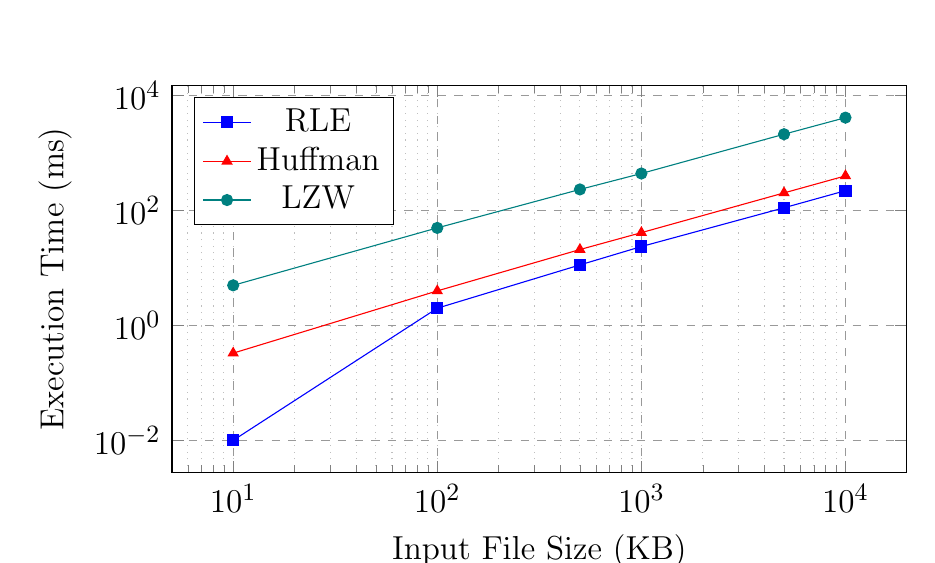
\begin{tikzpicture}
\begin{axis}[
    width=0.9\textwidth,
    height=6.5cm,
    xlabel={Input File Size (KB)},
    ylabel={Execution Time (ms)},
    xmode=log,
    ymode=log,
    log basis x={10},
    log basis y={10},
    grid=both,
    minor grid style={dotted,gray!50},
    major grid style={dashed,gray!80},
    legend pos=north west
]
\addplot[color=blue, mark=square*] coordinates {
    (10, 0.01) (100, 2.00) (500, 11.33) (1000, 23.67) (5000, 112.00) (10000, 222.33)
};
\addlegendentry{RLE}

\addplot[color=red, mark=triangle*] coordinates {
    (10, 0.33) (100, 4.00) (500, 21.00) (1000, 41.33) (5000, 203.33) (10000, 402.33)
};
\addlegendentry{Huffman}

\addplot[color=teal, mark=*] coordinates {
    (10, 5.00) (100, 50.00) (500, 233.67) (1000, 442.67) (5000, 2138.67) (10000, 4155.67)
};
\addlegendentry{LZW}
\end{axis}
\end{tikzpicture}
\caption{Execution Time Scaling vs. File Size on Log-Log Scale}
\label{fig:time_scaling}
\end{figure}

\subsection{Discussion \& Analytical Evaluation}

\subsubsection{Big-O Complexity vs. Empirical Growth Rate}
The empirical runtime curves in Figure~\ref{fig:time_scaling} closely corroborate the theoretical complexity models established in Section~3:
\begin{itemize}
    \item \textbf{RLE \& Huffman:} As input size $N$ scales by a factor of $10\times$ (e.g., $100\text{ KB} \to 1\text{ MB}$, and $1\text{ MB} \to 10\text{ MB}$), execution times scale strictly linearly by $\approx 10\times$ (from $2.00\text{ ms} \to 23.67\text{ ms} \to 222.33\text{ ms}$ for RLE; and $4.00\text{ ms} \to 41.33\text{ ms} \to 402.33\text{ ms}$ for Huffman). This confirms the $\mathcal{O}(N)$ bound.
    \item \textbf{LZW:} Exhibits higher constant factors ($\approx 10\times$ slower than Huffman). The lookup and insertion of string tokens into the dictionary create dynamic memory overhead and branch mispredictions, validating the empirical complexity of $\mathcal{O}(N \log K)$.
\end{itemize}

\subsubsection{Comparative Compression Ratio: Standard Prose vs. Highly Repetitive Data}
\begin{itemize}
    \item \textbf{Standard English Text:} LZW achieved the highest compression ratio ($2.60\times$), outperforming Huffman ($1.74\times$), while RLE suffered severe file inflation ($0.51\times$, a $96\%$ expansion).
    \item \textbf{Highly Repetitive Text:} LZW dominated with an exceptional ratio of $\mathbf{72.83\times}$, compared to Huffman ($3.32\times$) and RLE ($2.50\times$).
\end{itemize}

\subsubsection{Theoretical Justification of Results}
\begin{enumerate}
    \item \textbf{Single-Symbol Entropy Limit (Huffman):} Huffman operates strictly on zero-order entropy $H_0(S) = -\sum P(x)\log_2 P(x)$, assigning variable-length codes to independent symbols. Even in highly skewed prose, it cannot assign fewer than $1\text{ bit}$ per character, limiting its maximum theoretical compression ratio on ASCII text to $\approx 8 / 1.56 \approx 5.1\times$.
    \item \textbf{Multi-Character Dictionary Power (LZW):} LZW bypasses the single-symbol entropy bound by exploiting higher-order spatial redundancy. By progressively substituting multi-character phrases (e.g., repeating words or DNA motifs) with single 16-bit indices, a phrase of length $L$ yields an effective compression ratio of $\approx 8L / 16 = L/2$, leading to super-linear efficiency ($72.83\times$) on repetitive structures.
    \item \textbf{Incompressible Random Uniform Streams:} For cryptographic pseudo-random inputs ($H \approx 8.0\text{ bits/char}$), no statistical pattern or recurring substring exists. Huffman stagnates at $1.00\times$, while RLE ($0.50\times$) and LZW ($0.80\times$) introduce negative compression due to header metadata and unamortized multi-byte dictionary code indices.
\end{enumerate}

\cleardoublepage
\newpage

% ==================== 5. REFERENCES ====================
\section*{5. References}
\addcontentsline{toc}{section}{\numberline{}5. References}
\setcounter{section}{5}
\setcounter{subsection}{0}
\setcounter{subsubsection}{0}

\begin{itemize}
    \item[\textbf{[1]}] T. H. Cormen, C. E. Leiserson, R. L. Rivest, and C. Stein, ``Greedy Algorithms: Huffman Codes,'' in \emph{Introduction to Algorithms}, 3rd ed. Cambridge, MA, USA: MIT Press, 2009, ch. 16, sec. 3, pp. 428--437.
    \item[\textbf{[2]}] D. A. Huffman, ``A Method for the Construction of Minimum-Redundancy Codes,'' \emph{Proceedings of the IRE}, vol. 40, no. 9, pp. 1098--1101, Sept. 1952.
    \item[\textbf{[3]}] T. A. Welch, ``A Technique for High-Performance Data Compression,'' \emph{IEEE Computer}, vol. 17, no. 6, pp. 8--19, June 1984.
    \item[\textbf{[4]}] C. E. Shannon, ``A Mathematical Theory of Communication,'' \emph{The Bell System Technical Journal}, vol. 27, no. 3, pp. 379--423, July 1948.
    \item[\textbf{[5]}] J. Ziv and A. Lempel, ``A Universal Algorithm for Sequential Data Compression,'' \emph{IEEE Transactions on Information Theory}, vol. 23, no. 3, pp. 337--343, May 1977.
    \item[\textbf{[6]}] S. Khalid, \emph{Introduction to Data Compression}, 5th ed. Morgan Kaufmann, 2017.
\end{itemize}

\cleardoublepage
\newpage

% ==================== 6. ACKNOWLEDGEMENT ====================
\section*{6. Acknowledgement}
\addcontentsline{toc}{section}{\numberline{}6. Acknowledgement}
\setcounter{section}{6}
\setcounter{subsection}{0}
\setcounter{subsubsection}{0}

We would like to express our deepest gratitude to our course lecturers, \textbf{Assoc. Prof. Dr. Le Thanh Tung} and \textbf{Dr. Tran Hoang Quan} (Faculty of Information Technology, Department of Knowledge Engineering, HCMUS), for their dedicated lectures, rigorous feedback, and insightful academic guidance throughout this course.

Their instruction on computational complexity, dynamic data structures, and entropy bounds has established a solid theoretical foundation that enabled our team to execute this project effectively. 

In addition, AI tools, such as \textbf{ChatGPT} and \textbf{Gemini}, assisted with LaTeX document drafting, refining pseudocode representations, and formatting experimental trace tables. All core algorithm implementations, benchmarking datasets, and theoretical analyses were independently developed, validated, and verified by our team members.

Any remaining omissions or errors in this report are solely the responsibility of our group, and we warmly welcome all constructive critiques from the faculty.

\end{document}